% Format teze zasnovan je na paketu memoir
% http://tug.ctan.org/macros/latex/contrib/memoir/memman.pdf ili
% http://texdoc.net/texmf-dist/doc/latex/memoir/memman.pdf
% 
% Prilikom zadavanja klase memoir, navedenim opcijama se podešava 
% veličina slova (12pt) i jednostrano štampanje (oneside).
% Ove parametre možete menjati samo ako pravite nezvanične verzije
% mastera za privatnu upotrebu (na primer, u b5 varijanti ima smisla 
% smanjiti 
\documentclass[12pt,oneside]{memoir} 

% Paket koji definiše sve specifičnosti master rada Matematičkog fakulteta
\usepackage[latinica]{matfmaster} 

\usepackage[bottom]{footmisc}
\usepackage{latexsym}
\usepackage{amssymb}
\usepackage{amsmath}
%
% Podrazumevano pismo je ćirilica.
%   Ako koristite pdflatex, a ne xetex, sav latinički tekst na srpskom jeziku
%   treba biti okružen sa \lat{...} ili \begin{latinica}...\end{latinica}.
%
% Opicija [latinica]:
%   ako želite da pišete latiniciom, dodajte opciju "latinica" tj.
%   prethodni paket uključite pomoću: \usepackage[latinica]{matfmaster}.
%   Ako koristite pdflatex, a ne xetex, sav ćirilički tekst treba biti
%   okružen sa \cir{...} ili \begin{cirilica}...\end{cirilica}.
%
% Opcija [biblatex]:
%   ako želite da koristite reference na više jezika i umesto paketa
%   bibtex da koristite BibLaTeX/Biber, dodajte opciju "biblatex" tj.
%   prethodni paket uključite pomoću: \usepackage[biblatex]{matfmaster}
%
% Opcija [b5paper]:
%   ako želite da napravite verziju teze u manjem (b5) formatu, navedite
%   opciju "b5paper", tj. prethodni paket uključite pomoću: 
%   \usepackage[b5paper]{matfmaster}. Tada ima smisla razmisliti o promeni
%   veličine slova (izmenom opcije 12pt na 11pt u \documentclass{memoir}).
%
% Naravno, opcije je moguće kombinovati.
% Npr. \usepackage[b5paper,biblatex]{matfmaster}

% Pomoćni paket koji generiše nasumičan tekst u kojem se javljaju sva slova
% azbuke (nema potrebe koristiti ovo u pravim disertacijama)
\usepackage[latinica]{pangrami}

% Datoteka sa literaturom u BibTex tj. BibLaTeX/Biber formatu
\bib{matfmaster-primer}

% Ime kandidata na srpskom jeziku (u odabranom pismu)
\autor{Miloš P. Miković}
% Naslov teze na srpskom jeziku (u odabranom pismu)
\naslov{Algoritmi za rešavanje problema najkraće zajedničke nadniske}
% Godina u kojoj je teza predana komisiji
\godina{2021}
% Ime i afilijacija mentora (u odabranom pismu)
\mentor{dr Aleksandar \textsc{Kartelj}, docent\\ Univerzitet u Beogradu, Matematički fakultet}
% Ime i afilijacija prvog člana komisije (u odabranom pismu)
\komisijaA{dr Vladimir \textsc{Filipović}, redovni profesor\\ Univerzitet u Beogradu, Matematički fakultet}
% Ime i afilijacija drugog člana komisije (u odabranom pismu)
\komisijaB{dr Stefan \textsc{Mišković}, docent\\ Univerzitet u Beogradu, Matematički fakultet}
% Ime i afilijacija trećeg člana komisije (opciono)
% \komisijaC{}
% Ime i afilijacija četvrtog člana komisije (opciono)
% \komisijaD{}
% Datum odbrane (odkomentarisati narednu liniju i upisati datum odbrane ako je poznat)
% \datumodbrane{}

% Apstrakt na srpskom jeziku (u odabranom pismu)
\apstr{%
% \pangrami
}

% Ključne reči na srpskom jeziku (u odabranom pismu)
\kljucnereci{optimizacija, pretraga bima, analiza bioloških sekvenci}

\begin{document}
% ==============================================================================
% Uvodni deo teze
\frontmatter
% ==============================================================================
% Naslovna strana
\naslovna
% Strana sa podacima o mentoru i članovima komisije
\komisija
% Strana sa posvetom (u odabranom pismu)
\posveta{Hvala profesoru Aleksandru Kartelju.}
% Strana sa podacima o disertaciji na srpskom jeziku
\apstrakt
% Sadržaj teze
\tableofcontents*

% ==============================================================================
% Glavni deo teze
\mainmatter
% ==============================================================================

% ------------------------------------------------------------------------------
\chapter{Uvod}
% ------------------------------------------------------------------------------
% \pangrami
Problem najkraće zajedničke nadniske (\textit{eng.} Shortest Common Supersequence Problem)
jedan je od dobro poznatih NP-teških problema optimizacije u oblasti analize reči \cite{ProbabilisticBS}.
Ukratko, PNZN\footnote{U nastavku teksta PNZN ćemo koristiti kao skraćenicu za problem najkraće zajedničke nadniske}
se može opisati kao problem pronalaženja najkraće reči $\omega$ sačinjene
od simbola zadate konačne Azbuke $\Sigma$, tako da su sve sekvence iz unapred zadatog konačnog skupa
$\mathcal{L}$ sadržane u sekvenci $\omega$. Kada se kaže da su sve reči iz skupa $\mathcal{L}$
sadržane, misli se na to da se svaka reč iz skupa $\mathcal{L}$ može dobiti uklanjanjem simbola iz reči $\omega$ ali 
u zadatom redosledu \cite{SCSSProblemDef}. PNZN ima primene u mnogim oblastima informatike uključujući kompresiju podataka
\cite{DataCompression}, optimizaciju upita \cite{MQOptimization}, analizu i poređenje teksta i bioloških sekvenci \cite{ITAlgorithms} \cite{SeqComparison}.
Kao rezultat velike primene u mnogim oblastima, postoji veliki broj istraživanja na temu ovog problema u pokušaju da se dođe
do što boljeg i prihvatljivijeg rešenja.

\section{Problem najkraće zajedničke nadniske}
U ovom poglavlju formalno ćemo definisati PNZN, ali pre toga uvešćemo potrebnu notaciju koja će biti korišćena u nastavku
teksta. Konačna azbuku sastoji se od konačnog broja slova i označavaćemo je sa $\Sigma$. Svaka konačna reč
$\omega=\omega(1)\omega(2)...\omega(n)$ sastoji se od konačnog broja slova azbuke gde $\omega(j)\in\Sigma$ predstavlja j-to slovo reči $\omega\in\Sigma^*$.
Duzinu reči $\omega$ označavaćemo sa $|\omega|$, praznu reč sa $\varepsilon$ i važi da $|\varepsilon|=0$. U skladu sa uvedenom
notacijom $|\Sigma|$ predstavlja kardinalnost azbuke. Sa $\omega\unrhd\alpha$ označavaćemo broj pojavljivanja slova $\alpha$
u reči $\omega$ ($\omega(1)\omega(2)...\omega(n)\unrhd\alpha=\sum_{1<=i<=n,\omega(i)=\alpha}1$). Reč koja se dobija dodavanjem
slova $\alpha$ na početak reči $\omega$ označavaćemo sa $\alpha\omega$ (takođe ćemo pisati $\omega=\alpha\omega^{'}$), slično reč koja se dobija skidanjem slova $\alpha$ sa početka
reči $\omega$ sa $\omega|_{\alpha}$. Brisanje slova $\alpha$ sa početka svake reči u zadatom skupu, u skladu sa uvedenom notacijom
definišemo kao $\{\omega_{1},\omega_{2},...,\omega_{n}\}|_{\alpha}=\{\omega_{1}|_{\alpha},\omega_{2}|_{\alpha},...,\omega_{n}|_{\alpha}\}$.

Neka važi da $\omega_{1},\omega_{2}\in\Sigma^*$, za reč $\omega_{1}$ kažemo da je
supersekvenca reči $\omega_{2}$ u oznaci $\omega_{1}\succ\omega_{2}$ ako važi sledeća rekurzivna definicija \cite{ProbabilisticBS}:
\\
\\
\begin{equation}
\begin{aligned}
\omega_{1}\succ\varepsilon &\triangleq \textrm{Tačno}\\
\varepsilon\succ\omega_{2} &\triangleq \textrm{Netačno, \:\:Ako } \omega_{2}\neq\varepsilon\\
\alpha\omega_{1}\succ\alpha\omega_{2} &\triangleq \omega_{1}\succ\omega_{2}\\
\alpha\omega_{1}\succ\beta\omega_{2} &\triangleq \omega_{1}\succ\beta\omega_{2} \textrm{, \:\:Ako } \alpha\neq\beta
\end{aligned}
\end{equation}
\\

Zapravo, $\omega_{1}\succ\omega_{2}$ označava da se svi simboli iz $\omega_{2}$ nalaze u $\omega_{1}$ u datom redosledu,
ali ne nužno uzastopno. Na primer, za datu azbuku $\Sigma=\{a,c,t,g\}$, važi $agcatg \succ act$.
Sada možemo formalno definisati PNZN. Instanca PNZN može se definisati kao $\mathcal{I} =(\Sigma,\mathcal{L})$, gde 
$\Sigma$  predstavlja konačnu azbuku, a $\mathcal{L}$ predstavlja skup od $m$ reči $\{\omega_{1},\omega_{2},...,\omega_{m}\}$,
$\omega_{i}\in\Sigma^*$. Potrebno je pronaći reč $\omega$ najmanje dužine tako da važi da je $\omega$ supersekvenca svake reči iz
skupa $\mathcal{L}$ ($\omega\succ\omega_{i}, \forall\omega_{i}\in\mathcal{L} \textrm{ i } |\omega| \textrm{ je minimalna}$).
Na primer za instancu PNZN $\mathcal{I}=(\{a,c,t,g\},\{act,cta,aca\})$, najmanja zajednička supersekvenca
instance $\mathcal{I}$ je $acta$.  

\section{Pregled dosadašnjih istraživanja}
Problem najkraće zajedničke nadniske prvi je uveo Dejvid Mejer (\textit{eng.} David Maier) 1978. godine u svom radu 
"The Complexity of Some Problems on Subsequences and Supersequences" \cite{Maier}. Dokazano je da je PNZN NP-kompletan 
problem nad svakom azbukom $\Sigma$ za koju važi da $|\Sigma|\geqslant2$ \cite{NPComplete}. Korišćenjem dinamičkog
programiranja (\textit{eng.} dynamic programming) PNZN nad dve reči dužine $n$ rešen je algoritmom vremenske 
složenosti $\mathcal{O}(n^{2})$ i prostorne složenosti $\mathcal{O}(n^{2})$. Algortiam zasnovan na dinamičkom programiranju
može biti unapređen, pa tako za $k$ reči dužine maksimalno $n$, PNZN može biti rešen u $\mathcal{O}(n^{k})$ prostornoj i 
vremenskoj složenosti \cite{SCSDinamicProg}. Jasno je da ovakav algoritam nije praktičan za velike vrednosti $k$. S obzirom na to da ne postoji 
algoritam polinomijalne složenosti koji rešava PNZN, pribegava se optimizacionim metodama u rešavanju ovog problema.
Ono što je karakteristično za optimizacioni pristup rešavanju problema jeste to da se formira algoritam koji rešava
postojeći problem tako što daje rešenje koje je prihvatljivo pod određenim uslovima. Takvo rešenje ne mora nužno biti
optimalno rešenje problem. Na ovaj način, korišćenjem određene optimizacione tehnike, dobija se algoritam koji se izvršava
brzo u realnim uslovima i daje prihvatljivo dobra rešenja.

Vremenom je predloženo mnogo heurističkih i metaheurističkih algoritama za rešavanje PNZN.
Neke od poznatijih heurističkih funkcija koje su korišćene u rešavanju PNZN su Alphabet \cite{AlphabetSCS}, Majority Merge 
i Weighted Majority Merge \cite{ProbabilisticBS}, Tournament i Greedy \cite{Tournament}, Reduce-Expand \cite{AlphabetSCS}.
Pored navedenih funkcija, korišćeni su i metaheuristički algoritmi, genetski algoritam (\textit{eng.} genetic algorithm) \cite{SCSGenetic} i 
optimizacija kolonijom (\textit{eng.} colony optimization) \cite{SCSColony}, koji predstavljaju složenije optimizacione tehnike i imaju
tendenciju ka dužem vremenu izvršavanja ne većim instancama problema \cite{SCSSBetterSolution}.

Uvedi Beam search kao heuristiku koja ce biti koriscena u ovom radu.

% % Primeri citiranja\mathsf{Y} 
% Ovo je rečenica u kojoj se javlja citat \cite{PetrovicMikic2015}.
% Još jedan citat \cite{GuSh:243}.
% % Primeri navodnika
% Isprobavamo navodnike: "Rekao je da mu se javimo sutra".
% % Primer referisanja na tabelu (koja se javlja kasnije)
% U tabeli \ref{tbl:rezultati} koja sledi prikazani su rezultati eksperimenta.
% % Primer kraćeg ćiriličkog teksta
% {\cir Ово је пример ћириличког текста који се јавља у латиничком документу.}
% U ovoj rečenici se javlja jedna reč na {\cir ћирилици}.
% % Primer korišćenja fusnota
% % Iza ove rečenice sledi fusnota.\footnote{Ovo je fusnota.}

% % Primer dužeg ćirličkog teksta
% \begin{cirilica}
%   Ово је мало дужи блок текста исписан ћириличким писмом у оквиру
%   латиничког документа. Фијуче ветар у шибљу, леди пасаже и куће иза
%   њих и гунђа у оџацима.
% \end{cirilica}

% % Primer korišćenja tabele
% \begin{table}
% \centering
% \caption{Rezultati}
% \label{tbl:rezultati}
% \begin{tabular}{c>{\centering}p{2cm}c}
% \toprule
% 1 & 2 & 3\\\midrule
% 4 & 5 & 6\\\cmidrule(rl){1-2}
% 7 & 8 & 8\\
% \bottomrule
% \end{tabular}
% \end{table}

% % Primer korišćenja slike
% \begin{figure}[!ht]
%   \centering
%   \label{fig:grafikon}
%   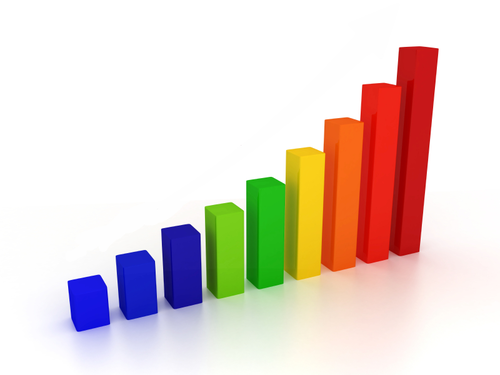
\includegraphics[width=0.5\textwidth]{graph.png}
%   \caption{Grafikon}
% \end{figure}


% % Primer jednostavnije matematičke formule
% Evo i jedan primer matematičke formule: $e^{i\pi} + 1 = 0$. 
% % Primer referisanja na sliku
% Na slici \ref{fig:grafikon} prikazan je jedan grafikon.

% % primer kompleksnije matematičke formule
% $$
% \int_a^b f(x)\ \mathrm{d}x \ =_{def}\ \lim_{\max{\Delta x_k \rightarrow 0}} \sum_{k=1}^n f(x_k^*)\Delta x_k
% $$

% % primer referisanja na poglavlja i strane poglavlja
% Više detalja biće dato u glavi \ref{chp:razrada} na strani \pageref{chp:razrada}.

% % primer liste
% Možemo praviti i nabrajanja:
% \begin{enumerate}
% \item Analiza 1
% \item Linearna algebra
% \item Analitička geometrija
% \item Osnovi programiranja
% \end{enumerate}

% \pangrami

% ------------------------------------------------------------------------------
\chapter{Razrada}
\label{chp:razrada}

% ------------------------------------------------------------------------------

% \pangrami

% \pangrami

% ------------------------------------------------------------------------------
\chapter{Zaključak}
% ------------------------------------------------------------------------------
% \pangrami

% \pangrami

% ------------------------------------------------------------------------------
% Literatura
% ------------------------------------------------------------------------------
\literatura

% ==============================================================================
% Završni deo teze i prilozi
\backmatter
% ==============================================================================

% ------------------------------------------------------------------------------
% Biografija kandidata
\begin{biografija}
  \textbf{Vuk Stefanović Karadžić} (\emph{Tršić,
    26. oktobar/6. novembar 1787. — Beč, 7. februar 1864.}) bio je
  srpski filolog, reformator srpskog jezika, sakupljač narodnih
  umotvorina i pisac prvog rečnika srpskog jezika.  Vuk je
  najznačajnija ličnost srpske književnosti prve polovine XIX
  veka. Stekao je i nekoliko počasnih mastera.  Učestvovao je u
  Prvom srpskom ustanku kao pisar i činovnik u Negotinskoj krajini, a
  nakon sloma ustanka preselio se u Beč, 1813. godine. Tu je upoznao
  Jerneja Kopitara, cenzora slovenskih knjiga, na čiji je podsticaj
  krenuo u prikupljanje srpskih narodnih pesama, reformu ćirilice i
  borbu za uvođenje narodnog jezika u srpsku književnost. Vukovim
  reformama u srpski jezik je uveden fonetski pravopis, a srpski jezik
  je potisnuo slavenosrpski jezik koji je u to vreme bio jezik
  obrazovanih ljudi. Tako se kao najvažnije godine Vukove reforme
  ističu 1818., 1836., 1839., 1847. i 1852.
\end{biografija}
% ------------------------------------------------------------------------------

\end{document}
